% This LaTeX was auto-generated from MATLAB code.
% To make changes, update the MATLAB code and export to LaTeX again.

\documentclass{article}

\usepackage[utf8]{inputenc}
\usepackage[T1]{fontenc}
\usepackage{lmodern}
\usepackage{graphicx}
\usepackage{color}
\usepackage{listings}
\usepackage{hyperref}
\usepackage{amsmath}
\usepackage{amsfonts}
\usepackage{epstopdf}
\usepackage[table]{xcolor}
\usepackage{matlab}

\sloppy
\epstopdfsetup{outdir=./}
\graphicspath{ {./dinteg_ddi_images/} }

\begin{document}

\label{H_6A01D316}
\matlabtitle{\underline{dinteg\_ddi}}

\begin{par}
\begin{flushleft}
performs the integral double of a sampled signal with the de-drifted integration (DDI method) 
\end{flushleft}
\end{par}

\matlabheading{\underline{Syntax}}

\begin{par}
\begin{flushleft}
\hyperref{845984F0}{pos=dinteg\_ddi(acc,freq)}
\end{flushleft}
\end{par}


\matlabheading{\underline{Description}}

\begin{par}
\begin{flushleft}
\texttt{pos=dinteg\_ddi(acc,freq)} performs the integral double of a signal \texttt{acc} sampled at \texttt{freq} Hz with the the optimally filtered integration (OFI method). 
\end{flushleft}
\end{par}

\begin{par}
\begin{flushleft}
It encompasses the subtraction of a weighted mean function of data samples, previous to each of both integrations. The acceleration drift function is computed by averaging a few initial and final accelerometry samples and by removing a lineal interpolation between both values from the original signal. The size of both sets of samples is empirically selected. 		
\end{flushleft}
\end{par}

\begin{par}
\begin{flushleft}
	  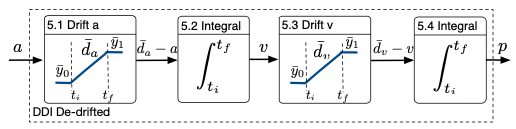
\includegraphics[width=\maxwidth{51.781234320120426em}]{image_0}		
\end{flushleft}
\end{par}

\begin{par}
\begin{flushleft}
The velocity drift function is based on the assumption of zero velocity at the beginning and end of the cycle, and a lineal function from zero to the mean of the last velocity samples is subtracted from to achieve it. 
\end{flushleft}
\end{par}

\begin{par}
\begin{flushleft}
More information: 
\end{flushleft}
\end{par}

\begin{par}
\begin{flushleft}
Rampp, A.; Barth, J.; Schuelein, S.; Gassmann, K.G.; Klucken, J.; Eskofier, B.M. Inertial Sensor-Based 							Stride Parameter Calculation From Gait Sequences in Geriatric Patients. \textit{IEEE Trans. Biomed. Eng. }\textbf{2015}, 							\textit{62}, 1089–1097. 												
\end{flushleft}
\end{par}


\matlabheading{\underline{Examples}}

\begin{matlabcode}
% cargamos datos de una acelerometro que sube y vuelve a la posicion de
% reposo:
filename='../simur_data/SAL.log';
datosxs=load(filename);
acc=datosxs(100:400,2)+9.8;
plot(acc);
\end{matlabcode}
\begin{center}
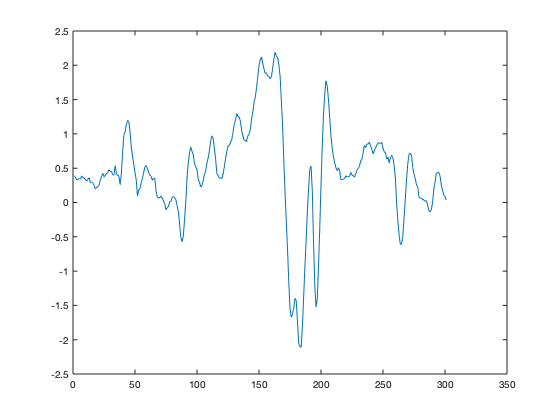
\includegraphics[width=\maxwidth{56.196688409433015em}]{figure_0.png}
\end{center}
\begin{matlabcode}
plot(dinteg_ofi(acc,100));
\end{matlabcode}
\begin{center}
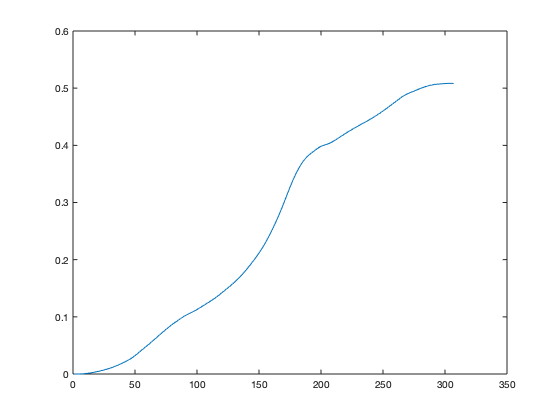
\includegraphics[width=\maxwidth{56.196688409433015em}]{figure_1.png}
\end{center}

\end{document}
